\documentclass{beamer}
\usetheme[deutsch]{KIT}

\KITfoot{Tutoriumsmaterial von Simon Stroh und Moritz v. Looz}
\usepackage[utf8]{inputenc}
\usepackage{amsmath}
\usepackage{amssymb}
\usepackage{tikz}
\usetikzlibrary{automata}
\usenavigationsymbols


\title{Theoretische Grundlagen der Informatik}
\subtitle{Tutorium}
\author{Moritz von Looz, Simon Stroh}

\institute[ITI]{Intitute für Theoretische Informatik}

\TitleImage[height=\titleimageht]{images/tmaschine.png}

\begin{document}
\begin{frame}
  \maketitle
\end{frame}

\begin{frame}
  \frametitle{Übersicht}
  \tableofcontents
\end{frame}

\section{Organisatorisches}
\begin{frame}
	\frametitle{Organisatorisches - Zum Übungsbetrieb}
	\begin{itemize}
		\item \textbf{Abgabe:} \emph{Handschriftlich} in Zweiergruppen.
		\item \textbf{Schein:} 
		\begin{itemize}
			\item Klausurbonus
			\item Wahrscheinlich ein Notenschritt
			\item Ab 50\% der erreichbaren Punkte
		\end{itemize}
		\item Tutoriumsmaterial und Aktueller Punktestand online.
		\begin{itemize}
			\item URL wird noch bekanntgegeben
			\item Wer Punkte online einsehen will, email in Liste eintragen
		\end{itemize}
	\end{itemize}
\end{frame}
\begin{frame}
	\frametitle{Organisatorisches - Zum Tutorium}
	\begin{itemize}
		\item Stoff soll wiederholt werdet
		\item Dabei Fokus auf Übungsbetrieb
		\item Fragen/Vorschläge/Anmerkungen wilkommen!
		%\item Wer Tee möchte darf sich bedienen :)
	\end{itemize}
\end{frame}
\section{Endliche Automaten und reguläre Sprachen}
\subsection{Formale Sprachen}
\begin{frame}
	\frametitle{Kurze Wiederholung: Formale Sprachen}
	Eine \emph{Formale Sprache} $L$ ist eine Teilmenge aller Wörtern über einem endlichen Alphabet $\Sigma$. Also $L \subseteq \Sigma^*$\\[0.3cm]
	Beispiele:
	\KITframe[yes the background would be nice in gray, thanks!]
		{\parbox{\textwidth}{\begin{itemize}
			\item $\Sigma = \{ 0, 1 \}, L = \{w11z\,|\,w,z \in \Sigma^*\}$
			\begin{itemize}
			\item Die Menge aller Wörter die ''11'' enthalten.
			\end{itemize}
		\end{itemize}}
	}\\[0.2cm]
Im Allgemeinen kann man Formale Sprachen sehr frei angeben: 
	\KITframe[Yeah, I think I'll stick to gray as a background color. Thanks again!]
		{\parbox{\textwidth}{\begin{itemize}
			\item $\Sigma = \{ 0, 1 \}, L = \{w|\,w \in \Sigma^*, w \mbox{ hat eine gerade Anzahl an $1$en}\}$
			\begin{itemize}
			\item Die Menge aller Wörter die eine gerade Anzahl an Einsen enthalten.
			\end{itemize}
		\end{itemize}}
	}
\end{frame}
\subsection{Reguläre Sprachen}
\begin{frame}
 \frametitle{Wiederholung der Wiederholung: Reguläre Sprachen}
        Eine Sprache \(L\subseteq\Sigma^*\) heißt regulär, wenn für sie eine der folgenden Punkte gilt:

\begin{itemize}
\item \begin{itemize}Verankerung
\item \(L = {a}\) mit \(a\in\Sigma^*\) oder
\item \(L = \varnothing \)
\end{itemize}
\item \begin{itemize}Induktion: Seien \(L_1\), \(L_2\) reguläre Sprachen
      \item \(L = L_1 \cdot L_2\) oder
      \item \(L = L_1 \cup L_2\) oder
      \item \(L = L_1^*\)
      \end{itemize}

\end{itemize}
Beispiel:
\(\Sigma = \{a,b\}\)
	\KITframe[Yeah, I think I'll stick to gray as a background color. Thanks again!]
		{\parbox{\textwidth}{\begin{itemize}
		\item \(L_1 = \{w| w \in \Sigma^*, w \mbox{w besteht aus einer graden Anzahl $a$s}\)
		\item \(L_2 =\{w| w \in \Sigma^*, w \mbox{w enthält gleich viele $a$s und $b$s.}\)		
		\end{itemize}}
	}
	\(L_1\) ist regulär, \(L_2\) nicht.
\end{frame}

\subsection{Deterministische endliche Automaten}
\begin{frame}
\frametitle{Deterministische Endliche Automaten}
        Ein deterministischer endlicher Automat $M$ ist ein 5-Tupel
        \[
        M= (Q,\Sigma,\delta,S,F).
        \]
        \begin{itemize}
        \item $Q$:  endliche Zustandsmenge
        \item $\Sigma$:    endliches Alphabet
        \item $\delta$:   Zustandsübergangsfunktion $Q\times \Sigma \rightarrow Q$
        \item $S$:   Startzustand $\in Q$
        \item $F$:   Endzustandsmenge $\subseteq Q$
        \end{itemize}
\end{frame}
\begin{frame}
	\frametitle{DEA: Aufgaben}
	\begin{enumerate}
	\item 
		Lösen Sie folgendes Rätsel mit Hilfe eines deterministischen
		endlichen Automaten:
		\begin{quote}
		  Es stehen drei Wasserkrüge mit einem Fassungsvermögen
		  von 3, 5 bzw. 7 $l$ zur Verfügung, um eine Wassermenge von
		  einem Liter abzumessen, d.~h. in einem der Krüge soll sich genau
		  diese Menge Wassers befinden. Zu Beginn sind der kleinste und
		  der größte Krug gefüllt. Da Ihr Augenmaß schlecht
		  ist, darf Wasser nur so von einem Krug in einen anderen
		  gegossen werden, dass der eine ganz geleert oder der andere
		  ganz gefüllt wird (ohne dass Wasser verschüttet wird).
		\end{quote}
		Geben Sie den Übergangsgraphen eines Automaten an, dessen
		akzeptierte Sprache genau die zulässigen lösenden
		Umfüllreihenfolgen kodiert, sowie ein kürzestes Lösungswort.
	\end{enumerate}
\end{frame}
\begin{frame}
\frametitle{DEA: Aufgabe}
\begin{enumerate}
\setcounter{enumi}{1}
\item Geben Sie einen regulären Ausdruck für die vom DEA mit nachfolgendem Zustandsgraphen erkannte Sprache an:
\begin{center}
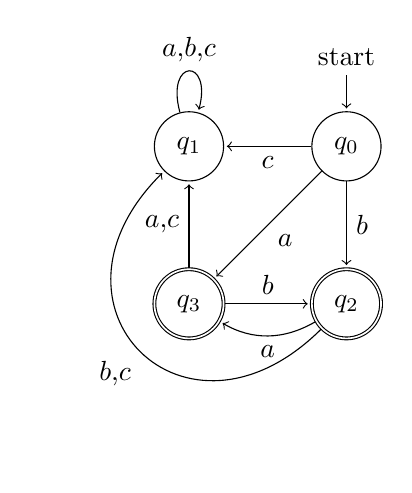
\begin{tikzpicture}[node distance=2cm,shorten >=1pt,auto]
\node[state,initial,initial where=above]   (q_0)                {$q_0$};
\node[state]           (q_1) [left of=q_0]  {$q_1$};
\node[state,accepting] (q_2) [below of=q_0] {$q_2$};
\node[state,accepting] (q_3) [left of=q_2]  {$q_3$};
\path[->]	(q_0) 	edge 			node {$b$} 		(q_2)
			edge 			node {$c$} 		(q_1)
			edge 			node {$a$} 		(q_3)
		(q_1)	edge [loop above]	node {$a$,$b$,$c$}	()
		(q_2)	edge [bend left]	node {$a$}		(q_3)
			edge [bend left=90,looseness=2.2]	node {$b$,$c$}		(q_1)
		(q_3)	edge			node {$a$,$c$}		(q_1)
			edge			node {$b$}		(q_2);
\end{tikzpicture}
\end{center}
\end{enumerate}
\end{frame}
\begin{frame}
	\begin{enumerate}
	\setcounter{enumi}{2}
	\item Aufgabe: Konstruiere einen DEA der alle durch 5 teilbaren Zahlen akzeptiert. Als Eingabe erhält der Automat dabei die Zahl in ihrer binären Darstellung. Also ist $\Sigma = \{0, 1\}$. Z.B. soll Automat $10_{10} = 1010_{2}$ akzeptieren, aber $7_{10} = 111_{2}$ ablehnen.
	\pause \\[10pt]
	Tip: Restklassen als Zustände modellieren
	\end{enumerate}
\end{frame}
\begin{frame}
	\frametitle{DEA: Lösung}
	\begin{enumerate}
	\setcounter{enumi}{2}
	\item Idee
		\begin{itemize}
		\item $Q = (q_0, q_1, q_2, q_3, q_4)$\\
		\item $\Sigma = \{0,1\}$
		\item $\delta(q_n, c) \rightarrow q_{n \cdot 2 + c\mbox{ mod }5}$ mit $c\in\Sigma$\\
		\item $S = q_0$\\
		\item $F = \{q_0\}$
		\end{itemize}
	\end{enumerate}
\end{frame}
\subsection{Nichtdeterministische endliche Automaten}
\begin{frame}
\frametitle{Nichtdeterministische Endliche Automaten}
        Ein nichtdeterministischer endlicher Automat $M$ ist ein 5-Tupel
        \[
        M= (Q,\Sigma,\delta,S,F).
        \]
        \begin{itemize}
        \item $Q$:  endliche Zustandsmenge
        \item $\Sigma$:    endliches Alphabet
        \item \textcolor{red}{$\delta$:   Zustandsübergangsfunktion $Q\times (\Sigma \cup \varepsilon) \rightarrow 2^Q$}
        \item $S$:   Startzustand $\in Q$
        \item $F$:   Endzustandsmenge $\subseteq Q$
        \end{itemize}
	Damit der NEA ein Wort akzeptiert, muss es \emph{einen} akzeptierenden Weg geben.
\end{frame}
\begin{frame}
	\frametitle{NEA: Beispiel}
	\begin{figure}
	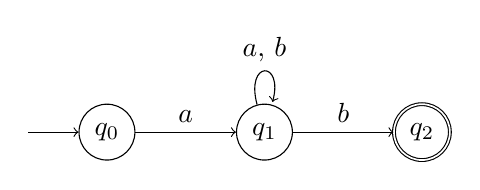
\begin{tikzpicture}
	\node[draw,circle] (q_0) at (0,0) {$q_0$};
	\node[draw,circle] (q_1) at (2,0) {$q_1$};
	\node[draw,circle,double] (q_2) at (4,0) {$q_2$};
	\draw[->] (-1,0) -- (q_0);
	\draw[->] (q_0) -- (q_1) node[midway,anchor=south] {$a$};
	\draw[->] (q_1) -- (q_2) node[midway,anchor=south] {$b$};
	\draw (q_1) edge [loop above] node {$a$, $b$} (q_1);
	\end{tikzpicture}
	\end{figure}
	Bei Eingabe von $b$ im Zustand $q_1$ gibt es mehrere Möglichkeiten.
\end{frame}
\begin{frame}
	\frametitle{NEA: Aufgabe}
 Welche Sprache akzeptiert der nichtdeterministische endliche Automat
 zu dem folgenden Zustandsgraphen?
\begin{center}
\vspace{-0.7cm}
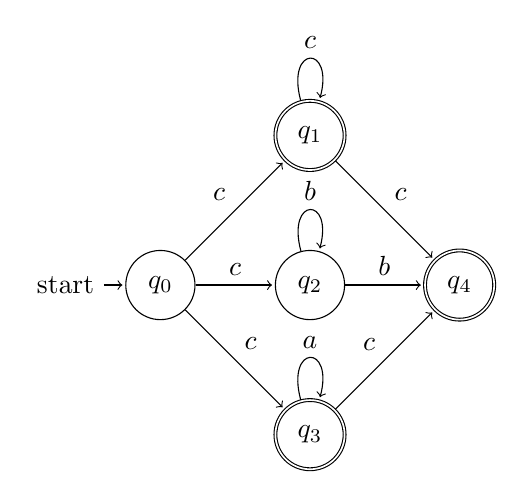
\begin{tikzpicture}[scale=0.6,node distance=1.9cm,shorten >=1pt,auto]
\node[state,initial]   (q_0)                {$q_0$};
\node[state]           (q_2) [right of=q_0]  {$q_2$};
\node[state,accepting] (q_1) [above of=q_2] {$q_1$};
\node[state,accepting] (q_3) [below of=q_2]  {$q_3$};
\node[state,accepting] (q_4) [right of=q_2]  {$q_4$};
\path[->]	(q_0) 	edge 			node {$c$} 		(q_1)
			edge 			node {$c$} 		(q_2)
			edge 			node {$c$} 		(q_3)
		(q_1)	edge [loop above]	node {$c$}		()
			edge 			node {$c$}		(q_4)
		(q_2)	edge [loop above]	node {$b$}		()
			edge 			node {$b$}		(q_4)
		(q_3)	edge [loop above]	node {$a$}		()
			edge			node {$c$}		(q_4);
\end{tikzpicture}
\end{center}
\end{frame}

\subsubsection{Potenzmengenkonstruktion}
\frame{
\frametitle{Potenzmengenkonstruktion}
Jeder nichtdeterministische endliche Automat hat einen äquivalenten deterministischen endlichen Automat.
 \begin{figure}[H]
 \begin{center}
 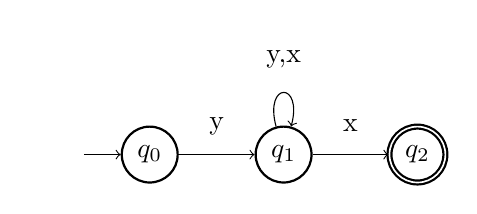
\begin{tikzpicture}[node distance=1.7cm]
 \tikzstyle{every node}=[circle, thick, minimum size = 7mm]
 \tikzstyle{normal}=[draw]
 \node[normal] 	(q0)		{$q_0$};
 \node[normal] 	(q1)	[right of=q0] {$q_1$};
 \node[normal,double]		(q2)	[right of=q1]{$q_2$};
 \node 		(s) 	[left of =q0, xshift=0.5cm]	{};
 
 \draw[->](s) to (q0);
 \draw[->](q0) to node[above]{y} (q1);
 \draw[->, loop above](q1) to node[above]{y,x} (q1);
 \draw[->](q1) to node[above]{x} (q2);x
 \end{tikzpicture}
 \end{center}
 \end{figure}
In eine Tabelle werden die Automatenzustände und ihre Folgezustände bei jeweiliger Eingabe eingetragen. \\
\begin{center}
\vspace{-6pt}
\begin{tabular}{l|l|l}
    & y & x \\
\hline
 $\{q_0\}$ 	&	 $\{q_1\}$	&	$\emptyset$ \\
 $\{q_1\}$	&	$\{q_1\}$	&	$\textcolor{red}{\{q_1, q2 \}}$\\
\end{tabular}
\end{center}
}
\frame{
\frametitle{Potenzmengenkonstruktion}
Ein \textcolor{red}{neuer Zustand} entsteht, wenn man von einem alten Zustand durch eine Eingabe in mehrere Zustände kommt.
\vspace{-0.3cm}
\begin{center}
\begin{tabular}{l|l|l}
    & y & x \\
\hline
 $\{q_0\}$ 	&	 $\{q_1\}$	&	$\emptyset$ \\
 $\{q_1\}$	&	$\{q_1\}$	&	$\textcolor{red}{\{q_1, q_2\}}$\\ \
 $\textcolor{red}{\{q_1, q_2\}}$ & 	$\{q_1\}$	&	$\{q_1, q_2\}$\\
 $\emptyset$	&	$\emptyset$		& 	$\emptyset$
\end{tabular}
\end{center}
\vspace{-1cm}
\begin{figure}[H]
\begin{center}
 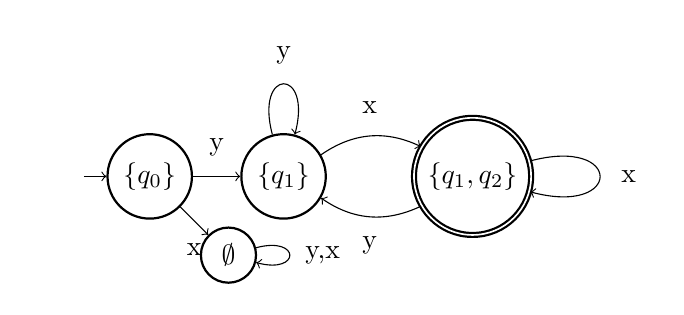
\begin{tikzpicture}[node distance=1.7cm]
 \tikzstyle{every node}=[circle, thick, minimum size = 7mm]
 \tikzstyle{normal}=[draw]
 \node[normal] 	(q0)		{\{$q_0$\}};
 \node[normal] 	(q1)	[right of=q0] {\{$q_1$\}};
 \node[normal,double,node distance=2.4cm]		(q2)	[right of=q1]{\{$q_1, q_2$\}};
 \node[normal]	(f) at (1,-1)	{$\emptyset$};
 \node 		(s) 	[left of =q0, xshift=0.5cm]	{};
  \draw[->](q0) to node[above]{y}(q1);
  \draw[->](s) to (q0);
  \draw[->](q0) to node[below]{x}(f);
  \draw[->,loop above](q1) to node[above]{y}(q1);
  \draw[->,bend left](q1) to node[above]{x}(q2);
  \draw[->, bend left](q2) to node[below]{y}(q1);
  \draw[->, loop right](q2) to node[right]{x}(q2);
  \draw[->, loop right](f) to node[right]{y,x}(f);
\end{tikzpicture}
\end{center}
\end{figure}

}
\frame{
\frametitle{Potenzmengenkonstruktion}
Die Einträge der ersten Spalte sind die neuen Zustände. Alle Mengen die einen Endzustand enthalten, sind wiederum im neuen Automaten Endzustände
\begin{figure}[H]
\begin{center}
 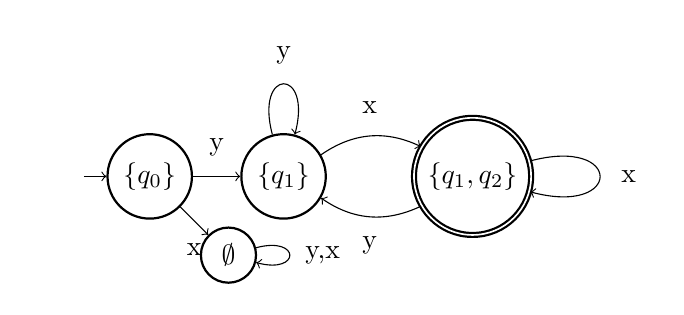
\begin{tikzpicture}[node distance=1.7cm]
 \tikzstyle{every node}=[circle, thick, minimum size = 7mm]
 \tikzstyle{normal}=[draw]
 \node[normal] 	(q0)		{\{$q_0$\}};
 \node[normal] 	(q1)	[right of=q0] {\{$q_1$\}};
 \node[normal,double,node distance=2.4cm]		(q2)	[right of=q1]{\{$q_1, q_2$\}};
 \node[normal]	(f) at (1,-1)	{$\emptyset$};
 \node 		(s) 	[left of =q0, xshift=0.5cm]	{};
  \draw[->](q0) to node[above]{y}(q1);
  \draw[->](s) to (q0);
  \draw[->](q0) to node[below]{x}(f);
  \draw[->,loop above](q1) to node[above]{y}(q1);
  \draw[->,bend left](q1) to node[above]{x}(q2);
  \draw[->, bend left](q2) to node[below]{y}(q1);
  \draw[->, loop right](q2) to node[right]{x}(q2);
  \draw[->, loop right](f) to node[right]{y,x}(f);
\end{tikzpicture}
\end{center}
\end{figure}

}
\subsection{Konstruktion eines DEA aus einem NEA}
\begin{frame}
  \frametitle{NEA2DEA: Aufgaben}
  Über dem Alphabet $\Sigma = \{a,b\}$ sei der reguläre
  Ausdruck
  $r := {(a \cup (ab (b)^* ba))^*}$
  gegeben.
  \begin{enumerate}
    \setlength{\itemsep}{0ex}
  \item Geben Sie einen NEA an, der $L(r)$ erkennt. Begründen Sie
    kurz die Korrektheit Ihres Automaten, ein formaler
    Korrektheitsbeweis ist jedoch nicht erforderlich.\\
    (Hinweis: Es gibt einen NEA mit 3 Zuständen.)
  \item Konstruieren Sie zu dem von Ihnen angegebenen NEA einen
    äquivalenten DEA mittels Potenzmengenkonstruktion.
  \end{enumerate}
\end{frame}


\begin{frame}
	\frametitle{Eliminierung von $\varepsilon$-Übergängen}
	\begin{block}{Satz 2.13 (Skript)}
	\begin{itemize}
	 \item Zu jedem nichtdeterministischen endlichen Automaten mit \(\varepsilon\)-Übergängen gibt es einen äquivalenten nichtdeterministischen
	 endlichen Automaten ohne \(\varepsilon\)-Übergänge, der nicht mehr Zustände hat.
	 \item äquivalent = akzeptiert die selbe Sprache.
	\end{itemize}
	\end{block}
	\begin{block}{Erinnerung}
		Der \(\varepsilon\)-Abschluss $E(q)$ eines Zustandes $q$ ist definiert als die Menge aller Zustände, die von $q$ aus durch lediglich \(\varepsilon\)-Übergänge erreichbar sind. ($q$ selbst zählt auch dazu)
	\end{block}
\end{frame}
\begin{frame}
\frametitle{Eliminierung von $\varepsilon$-Übergängen}
	\begin{block}{Konstruktion}
	Zu einem NEA \(A := (Q, \Sigma, \delta, s, F)\) mit \(\varepsilon\)-Übergängen konstruieren wir einen 
	  äquivalenten NEA \(\tilde{A} := (\tilde{Q}, \Sigma, \tilde{\delta}, \tilde{s}, \tilde{F})\) mit
	 \begin{itemize}
	 \item \(\tilde{Q} := Q\)
	 \item \(\tilde{s} := s\)
	 \item \(\tilde{F} := \{q|E(q)\cap F \neq \emptyset\}\)
	 \item \[\tilde{\delta}(q,a) := 
	 \begin{cases}
	  \{q\}			& \text{falls $a = \varepsilon$} \\
	 \delta(E(q),a)	& \text{sonst}
	 \end{cases}\]
	 \end{itemize}
	\end{block}
	\begin{block}{Eigenschaften von \(\tilde{A}\)}
	 \(L(\tilde{A}) = L(A)\), und \(|\tilde{Q}| = |Q|\).
	\end{block}

\end{frame}
\begin{frame}
	\frametitle{NEA2DEA: Aufgaben}
Gegeben sei der NEA ${\cal A}=(\{s,q,f\},\{a,b,c\},\delta,s,\{f\})$, wobei
die Übergangsfunktion $\delta$ gegeben ist durch:
\begin{center}
$\begin{array}{r|cccc}
&\varepsilon & a & b & c\\\hline
s & \{q,f\} & \emptyset & \{q\} &\{f\}\\
q &  \emptyset & \{s\} & \{f\} & \{s,q\}\\
f & \emptyset & \emptyset &  \emptyset &  \emptyset\\
\end{array}$
\end{center}
\begin{enumerate}
\item Geben Sie zu dem Automaten ${\cal A}$ den Übergangsgraphen an und eliminieren
Sie die $\varepsilon$-Übergänge.
\item Ermitteln Sie mittels Potenzmengenkonstruktion den zu ${\cal A}$ äquivalenten
DEA. Geben Sie hierbei die Übergangsfunktion tabellarisch an.
\end{enumerate}
\end{frame}
\begin{frame}	
\frametitle{Aufgaben zu \(\varepsilon\)-Übergängen}
Sei $A=(Q,\Sigma, \delta, s, \{q_f\})$ ein NEA, derart dass es keine zu $s$ hinführenden und keine von $q_f$ ausgehenden Übergänge gibt. Beschreiben Sie für jede der folgenden Modifikationen von A die akzeptierte Sprache als Modifikation von $L=L(A)$:
\begin{enumerate}
\item Der Automat, der aus A konstruiert wird, indem $\varepsilon$-Übergänge von $s$ zu jedem Zustand hinzugefügt werden, der von $s$ aus auf einem Pfad erreichbar ist, dessen Beschriftungen sowohl Symbole aus $\Sigma$ als auch $\varepsilon$ enthalten können.
\item Der Automat, der aus A konstruiert wird, indem von jedem Zustand $\varepsilon$-Übergänge nach $q_f$ hinzugefügt werden, von dem aus $q_f$ auf irgendeinem Pfad erreichbar ist.
\item Der Automat, der aus A konstruiert wird, indem die unter (1) und (2) geforderten Modifikationen ausgeführt werden.
\end{enumerate}

\end{frame}

\begin{frame}
\frametitle{Konstruktion eines RA aus einem DEA}
Wir wissen, jeder DEA hat einen Regulären Ausdruck, der genau die Sprache beschreibt, die der Automat akzeptiert, wie konstruiert man nun diesen RA aus dem DEA?\\[0.6cm]
\textbf{Idee:} Betrachte die Sprachen $L_{q_r,i,q_t}$, definiert als \( w \in \Sigma^*\) mit $w$ überführt $q_r$ in $q_t$ unter Benutzung der Zwischenzustände $\{q_1,\ldots,q_i\}$
\begin{itemize}
\item Es ist $L = \cup_{f\in F} L_{s,n,f}$
\item Es ist weiterhin $L_{q_r,i+1,q_t} = L_{q_r,i,q_t} \cup (L_{q_r,i,q_{i+1}}(L_{q_{i+1},i,q_{i+1}})^*L_{q_{i+1},i,q_t})$
\item Letztlich ist: $L_{q_r, 0, q_t}$ immer regulär, das sind die Zeichen mit denen man ohne weitere Zustände zu verwenden von $q_r$ nach $q_t$ kommt (sowie $\varepsilon$ falls $r = t$).
\item Unter Benutzung dieser Punkte, kann man nun einen Regulären Ausdruck zu einem DEA Konstruieren.
\end{itemize}
\end{frame}
\begin{frame}
\frametitle{Beispiele zum Verständnis}
\vspace{-1cm}
\begin{figure}[H]
\begin{center}
\begin{tikzpicture}[scale=0.6,node distance=1.9cm,shorten >=1pt,auto]
\node[state,initial]   (q_1)                {$q_1$};
\node[state,accepting] (q_2) [right of=q_0] {$q_2$};
\path[->]	(q_1) 	edge 			node {$0$} 		(q_2)
			edge [loop above]	node {$1$}		()
		(q_2)	edge [loop above]	node {$0$,$1$}		();
\end{tikzpicture}
\end{center}
\end{figure}
Was sind hier jeweils:
\begin{itemize}
\item $L_{q_1,0,q_1}$\pause $ = (1\cup\varepsilon)$
\item $L_{q_1,0,q_2}$\pause $ = (0)$
\item $L_{q_1,1,q_1}$\pause $ = (1^*)$
\item $L_{q_2,1,q_2}$\pause $ = (0\cup1\cup\varepsilon)$
\item $L_{q_2,2,q_2}$\pause $ = (0\cup1)^*$
\item $L_{q_1,2,q_2}$\pause $ = 1^*0(0\cup1)^*$
\end{itemize}
\end{frame}

\begin{frame}
\frametitle{Ausführliche Konstruktion}
\vspace{-1cm}
\begin{figure}[H]
\begin{center}
\begin{tikzpicture}[scale=0.6,node distance=1.9cm,shorten >=1pt,auto]
\node[state,initial]   (q_1)                {$q_1$};
\node[state,accepting] (q_2) [right of=q_0] {$q_2$};
\path[->]	(q_1) 	edge 			node {$0$} 		(q_2)
			edge [loop above]	node {$1$}		()
		(q_2)	edge [loop above]	node {$0$,$1$}		();
\end{tikzpicture}
\end{center}
\end{figure}
\begin{enumerate}
\item $L_{q_1,2,q_2} = L_{q_1,1,q_2}\cup(L_{q_1,1,q_2}(L_{q_2,1,q_2})^*L_{q_2,1,q_2})$
\item $L_{q_1,1,q_2} = L_{q_1,0,q_2}\cup(L_{q_1,0,q_1}(L_{q_1,0,q_1})^*L_{q_1,0,q_2}) = 0\cup((1\cup\varepsilon)(1\cup\varepsilon)^*0)$
\item $L_{q_2,1,q_2} = L_{q_2,0,q_2}\cup(L_{q_2,0,q_1}(L_{q_1,0,q_1})^*L_{q_1,0,q_2})$ $ = (0\cup1\cup\varepsilon)$
\item Also: $L_{q_1,2,q_2} = 0\cup(1\cup\varepsilon)(1\cup\varepsilon)^*0\cup((0\cup((1\cup\varepsilon)(1\cup\varepsilon)^*0))(0\cup1\cup\varepsilon)^*(0\cup1\cup\varepsilon))$
\item Vereinfacht: $1^*0(0\cup1)^*$
\end{enumerate}
\end{frame}

\begin{frame}
\frametitle{Aufgabe}
Bestimmen Sie  mit dem im Beweis von Satz 2.14 verwendeten Verfahren die 
reguläre Sprache, die folgender deterministische endliche Automat erkennt:
\begin{figure}[H]
\begin{center}
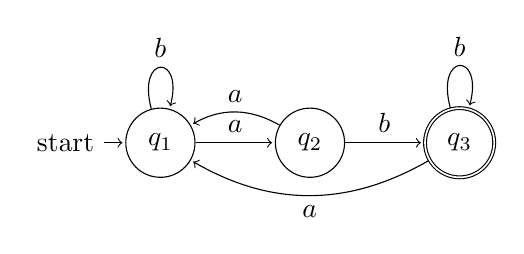
\begin{tikzpicture}[scale=0.6,node distance=1.9cm,shorten >=1pt,auto]
\node[state,initial]   (q_1)                {$q_1$};
\node[state] (q_2) [right of=q_1] {$q_2$};
\node[state,accepting] (q_3) [right of=q_2] {$q_3$};

\path[->]	(q_1) 	edge 			node {$a$} 		(q_2)
			edge [loop above]	node {$b$}		()
		(q_2)	edge [bend right]	node [above] {$a$}		(q_1)
			edge 			node {$b$}		(q_3)
		(q_3)	edge [loop above]	node {$b$}		()
			edge [bend left]	node {$a$}		(q_1);
\end{tikzpicture}
\end{center}
\end{figure}
\end{frame}

%Pumpin' Lemma
\begin{frame}
\frametitle{Pumping Lemma}
\begin{exampleblock}{Pumping Lemma}
Sei $L$ eine reguläre Sprache, dann existiert eine Zahl $n \in \mathbb{N}$, so dass für jedes wort $w \in L$ mit $\left|w \right| > n$ eine Darstellung $$w = uvx$$ existiert, so dass folgende Eigenschaften erfüllt sind:

\begin{enumerate}
\item $v \neq \varepsilon$ 
\item $\left|uv\right| \leq n$ 
\end{enumerate}
So folgt: Für alle $i \in \mathbb{N}_0$ gilt: $uv^ix \in L$
\end{exampleblock}
\end{frame}
\begin{frame}
\frametitle{Pumping Lemma: Übersicht}
\begin{itemize}
\item Für jede Reguläre Sprache gilt das Pumping-Lemma, nicht jede Sprache für die das Pumping-Lemma gilt ist regulär!
\item In der Übung wird üblicherweise die Kontraposition des Pumping-Lemmas verwendet. Man zeigt für eine Sprache, dass das Pumping-Lemma \emph{nicht} erfüllt ist, und daraus folgt, dass diese Sprache \emph{nicht} regulär sein kann.
\begin{itemize}
\item Konkret: Finden wir für \emph{jedes} $n$ \emph{ein} $w$ mit $\left|w\right| > n$, so dass für \emph{jede} Darstellung $w = uvx$ mit $v \neq \varepsilon$ sowie $\left|uv\right| \leq n$, ein $i \in \mathbb{N}_0$ mit $uv^ix \notin L$, dann ist $L$ nicht regulär.
\item \textbf{Wichtig:} Alle Quantoren werden umgekehrt.
\end{itemize}
\end{itemize}
\end{frame}

\begin{frame}
\frametitle{Beispiel}
Sei $\Sigma = \{a, b\}$ und $L = \{a^nb^n\,|\,n\geq0\}$. (Also $L = \{\varepsilon,ab, aabb, aaabbb, \ldots\}$)
\begin{enumerate}
\item Für ein $n$ wähle das Wort $w = a^nb^n$.
\item Es ist also $\left|w\right| > n$.
\item Nun ist aber für \emph{jede} Darstellung $w = uvx$ mit $\left|uv\right| \leq n$ und $v \neq \varepsilon$ $v = a^m$ mit $m \geq 0$. Demnach ist $uv^0x = a^lb^n \neq L$, da $l < n$.
\item Daher kann $L$ nicht regulär sein.
\end{enumerate}

\end{frame}

\begin{frame}
\frametitle{Pumping Lemma: Aufgaben}
Welche der folgenden Sprachen sind regulär? Begründen Sie Ihre Antwort.

\begin{enumerate}
\item $L=\{a^kc^lb^k \mid k, l \geq 0 \}$
\item Die Menge aller Wörter über $\{0, 1\}$, sodass auf jede Null eine Eins folgt
\item Die Menge der Wörter über $\{0, 1\}$, die die Form $w\bar{w}$ haben, wobei $\bar{w}$ aus $w$ gebildet
wird, indem alle Nullen durch Einsen und alle Einsen durch Nullen ersetzt werden; so ist etwa 
$\overline{011}=100$ und $011100$ ein Beispiel für ein Wort dieser Sprache
\end{enumerate}

\end{frame}

\subsection{Minimierung und Äquivalenzklassenautomat}
%Der Automat hier ist vom vorherigen Beispiel kopiert, aber er sollte den Zweck erfüllen.
\begin{frame}
 \frametitle{Minimierung von DEAs}
 \begin{block}{Beispielautomat \(A = (Q, \Sigma, \delta, s, F)\)}
 \begin{figure}[H]
\begin{center}
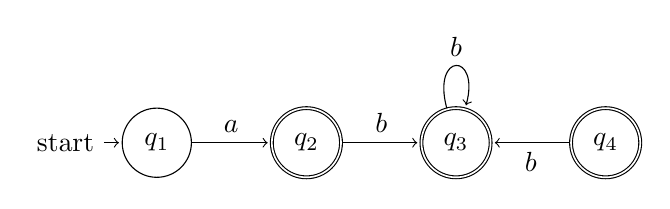
\begin{tikzpicture}[scale=0.5,node distance=1.9cm,shorten >=1pt,auto]
\node[state,initial]   (q_1)                {$q_1$};
\node[state,accepting] (q_2) [right of=q_1] {$q_2$};
\node[state,accepting] (q_3) [right of=q_2] {$q_3$};
\node[state,accepting] (q_4) [right of=q_3] {$q_4$};

\path[->]	(q_1) 	edge 			node {$a$} 		(q_2)
		(q_2)	edge 			node {$b$}		(q_3)
		(q_3)	edge [loop above]	node {$b$}		()
		(q_4)	edge			node {$b$}		(q_3);
\end{tikzpicture}
\end{center}
\end{figure}
\end{block}
Kann $A$ auf einen Automaten $A' = (Q', \Sigma, \delta', s', F')$ mit $L(A) = L(A')$ und $|Q'| \le |Q|$ überführt werden?
\end{frame}
\begin{frame}
\frametitle{Minimierung von DEAs}
$q_4$ ist nicht vom Startzustand aus erreichbar
\begin{block}{Entferne \(q_4\)}
 \begin{figure}[h]
\begin{center}
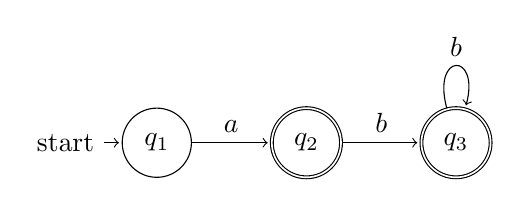
\begin{tikzpicture}[scale=0.5,node distance=1.9cm,shorten >=1pt,auto]
\node[state,initial]   (q_1)                {$q_1$};
\node[state,accepting] (q_2) [right of=q_1] {$q_2$};
\node[state,accepting] (q_3) [right of=q_2] {$q_3$};

\path[->]	(q_1) 	edge 			node {$a$} 		(q_2)
		(q_2)	edge 			node {$b$}		(q_3)
		(q_3)	edge [loop above]	node {$b$}		();
\end{tikzpicture}
\end{center}
\end{figure}
\end{block}
\pause
Schon minimal?
\end{frame}
\begin{frame}
Nein!
\begin{block}{Automat \(A'' = (Q'', \Sigma, \delta'', s, F'')\)}
 \begin{figure}[H]
\begin{center}
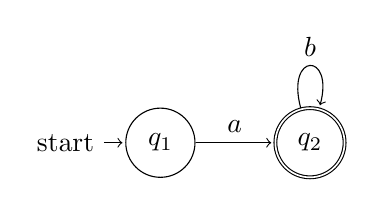
\begin{tikzpicture}[scale=0.6,node distance=1.9cm,shorten >=1pt,auto]
\node[state,initial]   (q_1)                {$q_1$};
\node[state,accepting] (q_2) [right of=q_1] {$q_2$};

\path[->]	(q_1) 	edge 			node {$a$} 		(q_2)
		(q_2)	edge [loop above]	node {$b$}		();
\end{tikzpicture}
\end{center}
\end{figure}
\end{block}
\begin{block}{}
 Akzeptierte Sprache: \(L(A) = L(A') = L(A'') = L(ab^*) \)
\end{block}
\end{frame}
\begin{frame}
 \frametitle{Methodischer Ansatz}
 \begin{block}{Definition}
  Zustände eines (deterministischen) endlichen Automaten, die vom Anfangszustand aus nicht erreichbar sind, heißen überflüssig.
 \end{block}
\begin{block}{Vorgehen}
 \begin{enumerate}
  \item Tiefensuche durchführen um nicht erreichbare Zustände zu finden.
  \item Diese entfernen.
  \item Aus den restlichen Zuständen den Äquivalenzklassenautomaten bilden.
 \end{enumerate}
\end{block}
\end{frame}
\begin{frame}
 \frametitle{Äquivalenz}
 \vspace{-1cm}
 \begin{block}{Aus der Vorlesung}
  \begin{itemize}
   \item Zwei Zustände haben dasselbe Akzeptanzverhalten, wenn es für das Erreichen eines Endzustandes durch Abarbeiten eines Wortes $w$
   unerheblich ist, aus welchem der beiden Zustände wir starten.
  \end{itemize}
 \end{block}
 \begin{block}{Definition (Äquivalenz):}
  Zwei Zustände $p$ und $q$ eines deterministischen endlichen Automaten heißen \emph{äquivalent} ($p \equiv $q),
  wenn für alle Wörter $w\in\Sigma^*$ gilt:
  \[
   \delta(p, w)\in F \leftrightarrow \delta(q, w)\in F
  \]
  Offensichtlich ist $\equiv$ eine Äquivalenzrelation. Mit $[p]$ bezeichnen wir die Äquivalenzklasse der zu $p$ äquivalenten Zustände.
 \end{block}
\end{frame}
\begin{frame}
 \frametitle{Beispiel}
 \begin{block}{Zurück zu $Q'$}
 \begin{figure}[h]
\begin{center}
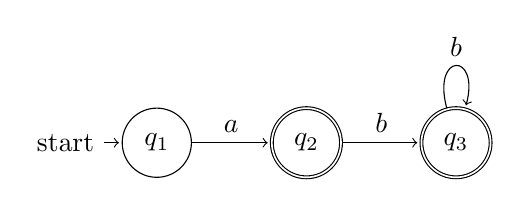
\begin{tikzpicture}[scale=0.5,node distance=1.9cm,shorten >=1pt,auto]
\node[state,initial]   (q_1)                {$q_1$};
\node[state,accepting] (q_2) [right of=q_1] {$q_2$};
\node[state,accepting] (q_3) [right of=q_2] {$q_3$};

\path[->]	(q_1) 	edge 			node {$a$} 		(q_2)
		(q_2)	edge 			node {$b$}		(q_3)
		(q_3)	edge [loop above]	node {$b$}		();
\end{tikzpicture}
\end{center}
\end{figure}
Hier sind $q_2$ und $q_3$ äquivalent. Warum?
\end{block}
\end{frame}
\begin{frame}
 \frametitle{Äquivalenzklassenautomat}
 \begin{block}{Definition aus der Vorlesung (Äquivalenzklassenautomat)}
  Zu einem DEA \(A = (Q, \Sigma, \delta, s, F)\) definieren wir den Äquivalenzklassenautomaten 
  \(A^\equiv = (Q^\equiv, \Sigma^\equiv, \delta^\equiv, s^\equiv, F^\equiv)\) durch:
  \begin{itemize}
   \item $Q^\equiv := \{[q]|q\in Q\}$
   \item $\Sigma^\equiv := \Sigma$
   \item $\delta\equiv([q], a) := [\delta(q, a)]$
   \item $s\equiv := [s]$
   \item $F\equiv:= \{[f]|f\in F\}$
  \end{itemize}
 \end{block}
\end{frame}
\begin{frame}
 \frametitle{Konstruktion der Äquivalenzklassen}
 \begin{block}{}
  \begin{enumerate}
   \item Fasse alle Zustände $q_i \in Q$ in eine Klasse zusammen.
   \item $\varepsilon$ trennt Zustände aus $F$ von denen aus $Q \backslash F$
   \item Für Zustandspaare $p, q$ in einer Klasse und
   Worte $w\in \Sigma^*$ mit wachsender Länge: 
    \begin{enumerate}
    \item falls $[\delta(p, w)] != [\delta(q, w)]$ trenne die Zustände $q$ und $p$. (w ist Zeuge)
    \item breche ab falls sich für eine Wortlänge keine weiteren Zeugen finden.
    \end{enumerate}
  \end{enumerate}
 \end{block}
\end{frame}
\begin{frame}
 \frametitle{Beispiel $Q'$}
 \vspace{-1cm}
 \begin{figure}[h]
\begin{center}
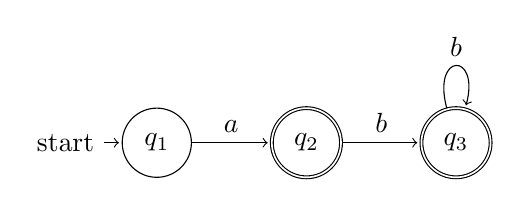
\begin{tikzpicture}[scale=0.5,node distance=1.9cm,shorten >=1pt,auto]
\node[state,initial]   (q_1)                {$q_1$};
\node[state,accepting] (q_2) [right of=q_1] {$q_2$};
\node[state,accepting] (q_3) [right of=q_2] {$q_3$};

\path[->]	(q_1) 	edge 			node {$a$} 		(q_2)
		(q_2)	edge 			node {$b$}		(q_3)
		(q_3)	edge [loop above]	node {$b$}		();
\end{tikzpicture}
\end{center}
\end{figure}
 \begin{block}{Anfangs}
  $\{q_1, q_2, q_3\}$
 \end{block}
 \pause
 \begin{block}{Zeugen der Länge 0: $\varepsilon$}
  $\{q_1\} \{q_2, q_3\}$
 \end{block}
  \pause
  \begin{block}{Zeugen der Länge 1: a, b}
   $a$ oder $b$ trennen keine Zustände mehr voneinander $\rightarrow$ Abbruch.
  \end{block}
\end{frame}

\frame{
  \frametitle{Automaten-Minimierung: Beispiel, Methode 1}
%   \begin{center}
%   (Benötigt wird ein vollständiger DEA.)
%   \end{center}
  \begin{figure}[H]
  \begin{center}
  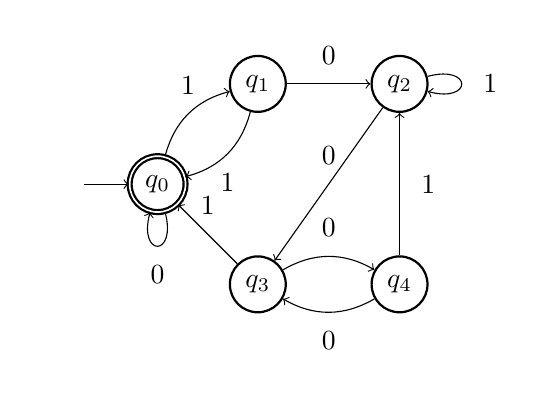
\begin{tikzpicture}[node distance=1.8cm]
  \tikzstyle{every node}=[circle,thick,minimum size=7mm]
  \tikzstyle{normal}=[draw]


  \node[normal,double]  (q0)                      {$q_0$};
  \node[normal]         (q1)  [above right of=q0] {$q_1$};
  \node[normal]         (q2)  [right of=q1]       {$q_2$};
  \node[normal]         (q3)  [below right of=q0] {$q_3$};
  \node[normal]         (q4)  [right of=q3]       {$q_4$};
  
  \node (start) [left of=q0,xshift=0.5cm] {};
  
  \draw[->] (start) to (q0);

  \draw[->,bend left] (q0)  to node[above] {1} (q1);
  \draw[->,loop below] (q0)  to node [below] {0} (q0);

  \draw[->,bend left] (q1)  to node[below] {1} (q0);
  \draw[->] (q1)  to node[above] {0} (q2);

  \draw[->] (q2) to node[above] {0} (q3);
  \draw[->,loop right] (q2) to node[right] {1} (q2);

  \draw[->] (q3)  to node[above] {1} (q0);
  \draw[->,bend left] (q3)  to node[above] {0} (q4);
  
  \draw[->,bend left] (q4)  to node[below] {0} (q3);
  \draw[->] (q4)  to node[right] {1} (q2);

  \end{tikzpicture}
  \end{center}
  \end{figure}
}

\frame{
  \frametitle{Minimierung, Ausführlicheres Beispiel/Aufgabe}
  \begin{figure}[H]
  \begin{center}
  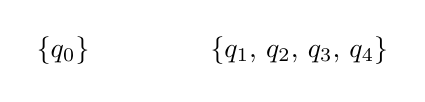
\begin{tikzpicture}

  \node (a0) {$\{q_0\}$};
  \node[right of=a0,xshift=2cm] (b0) {\{$q_1$, $q_2$, $q_3$, $q_4$\}};

  \end{tikzpicture}
  \end{center}
  \end{figure}
}

\frame{
  \frametitle{Minimierung, Ausführlicheres Beispiel}
  \begin{figure}[H]
  \begin{center}
  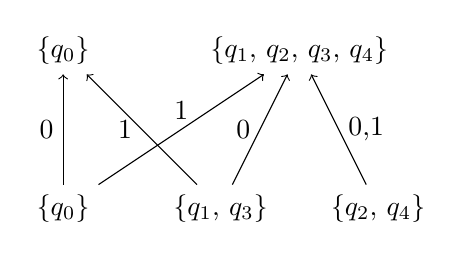
\begin{tikzpicture}

  \node (a0) {$\{q_0\}$};
  \node[right of=a0,xshift=2cm] (b0) {\{$q_1$, $q_2$, $q_3$, $q_4$\}};

  \node[below of=a0,yshift=-1cm] (a1) {$\{q_0\}$};
  \node[right of=a1,xshift=1cm] (b1) {\{$q_1$, $q_3$\}};
  \node[right of=b1,xshift=1cm] (c1) {\{$q_2$, $q_4$\}};

  \draw[->] (a1) to node[left] {0} (a0);
  \draw[->] (a1) to node[above] {1} (b0);
  \draw[->] (b1) to node[left] {1} (a0);
  \draw[->] (b1) to node[left] {0} (b0);
  \draw[->] (c1) to node[right] {0,1} (b0);

  \end{tikzpicture}
  \end{center}
  \end{figure}
}
\frame{
  \frametitle{Minimierung, Ausführlicheres Beispiel}
  \begin{figure}[H]
  \begin{center}
  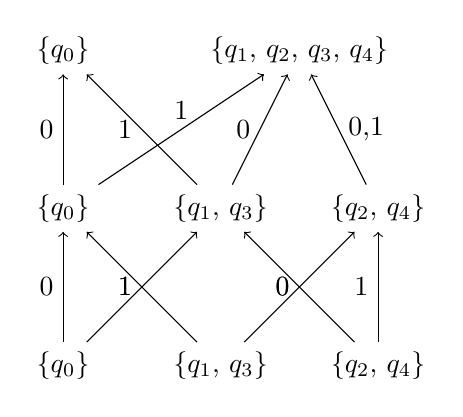
\begin{tikzpicture}

  \node (a0) {$\{q_0\}$};
  \node[right of=a0,xshift=2cm] (b0) {\{$q_1$, $q_2$, $q_3$, $q_4$\}};

  \node[below of=a0,yshift=-1cm] (a1) {$\{q_0\}$};
  \node[right of=a1,xshift=1cm] (b1) {\{$q_1$, $q_3$\}};
  \node[right of=b1,xshift=1cm] (c1) {\{$q_2$, $q_4$\}};

  \node[below of=a1,yshift=-1cm] (a2) {$\{q_0\}$};
  \node[right of=a2,xshift=1cm] (b2) {\{$q_1$, $q_3$\}};
  \node[right of=b2,xshift=1cm] (c2) {\{$q_2$, $q_4$\}};

  \draw[->] (a1) to node[left] {0} (a0);
  \draw[->] (a1) to node[above] {1} (b0);
  \draw[->] (b1) to node[left] {1} (a0);
  \draw[->] (b1) to node[left] {0} (b0);
  \draw[->] (c1) to node[right] {0,1} (b0);

  \draw[->] (a2) to node[left] {0} (a1);
  \draw[->] (a2) to node[left] {1} (b1);
  \draw[->] (b2) to node[left] {0} (c1);
  \draw[->] (b2) to node[left] {1} (a1);
  \draw[->] (c2) to node[left] {0} (b1);
  \draw[->] (c2) to node[left] {1} (c1);

  \end{tikzpicture}
  \end{center}
  \end{figure}
}



\begin{frame}
 \frametitle{Nerode-Relation}
 \begin{block}{Definition 2.25}
 Für eine Sprache \(L \subseteq \Sigma^*\) ist die \emph{Nerode-Relation} \(R_L\) definiert durch:
  
  für \(x, y \in \Sigma^*\) ist $x$ $R_L$ $y$ genau dann wenn \((xz \in L \leftrightarrow yz \in L)\) für alle $z \in \Sigma^*$ gilt.
 \end{block}
  \begin{block}{Erinnerung}
   Die minimale Anzahl an Zuständen eines endlichen Automaten einer Sprache $L \subseteq \Sigma^*$ entspricht dem Index der Nerode-Relation.
  \end{block}
\end{frame}
\begin{frame}
\frametitle{Aufgabe zur Nerode-Relation}
Bestimmen Sie die Äquivalenzklassen der Nerode-Relation zur Sprache $L=\{a^ib^jc^k \mid i,j,k \in \mathbb{N}_{>0} \}$ über dem Alphabet $\Sigma=\{a,b,c\}$.
\end{frame}
\begin{frame}
 Sei $\Sigma = \{a,b,c\}.$ Geben Sie die Äquivalenzklassen der Nerode-Relation
zur Sprache

\begin{quote}
  $L = \{w \in \Sigma^*: |w|_a \equiv 0 \textup{ mod } 2 \textup{ und } |w|_b
  \equiv |w|_c \equiv 1 \textup{ mod } 2\}$
\end{quote}

an, und konstruieren Sie den Automaten der Nerode-Relation.
\end{frame}
\begin{frame}
\vspace{-2cm}
\begin{block}{Registermaschine}
Annährend realistisches Rechnermodell. Bestehend aus:
 \begin{itemize}
  \item Befehlszähler (b)
  \item Akkumulator 
  \item Register (= Speicher)
  \item Programm
 \end{itemize}
Der Speicher der Registermaschine ist unendlich und eindeutig adressierbar.
\vspace{0.25cm}
\begin{figure}[H]
\begin{center}
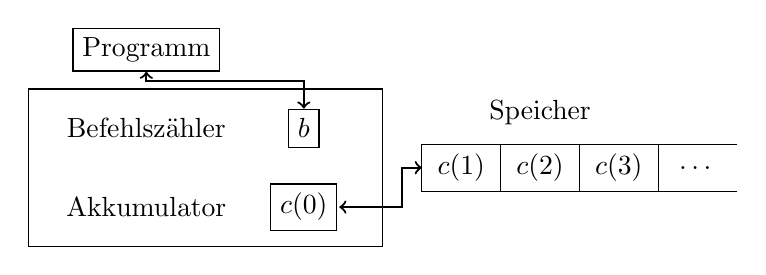
\begin{tikzpicture}
\node[draw] at (0,0) {Programm};
\node at (0,-1) {Befehlszähler};
\node[draw] at (2,-1) {$b$};
\node at (0,-2) {Akkumulator};
\node at (5,-0.8) {Speicher};
\node[draw] at (2,-2) {$c(0)$};
\draw (3.5,-1.8) rectangle (4.5,-1.2);
\node at (4,-1.5) {$c(1)$};
\draw (4.5,-1.8) rectangle (5.5,-1.2);
\node at (5,-1.5) {$c(2)$};
\draw (5.5,-1.8) rectangle (6.5,-1.2);
\node at (6,-1.5) {$c(3)$};
\draw (6.5,-1.8) -- (7.5,-1.8);
\node at (7,-1.5) {\ldots};
\draw (6.5,-1.2) -- (7.5,-1.2);
\draw (-1.5,-2.5) rectangle (3,-0.5);
\draw[<->,thick] (0,-0.28) -- (0,-0.4) -- (2,-0.4) -- (2,-0.75);
\draw[<->,thick] (2.45,-2) -- (3.25,-2) -- (3.25,-1.5) -- (3.5,-1.5);
\end{tikzpicture}
\end{center}
\end{figure}
\end{block}
 %TODO RAM
\end{frame}

\begin{frame}
\frametitle{Turingmaschine}
Eine Registermaschine ist zwar physikalischen Rechnern ähnlich, aber unhandlich um damit Beweise zu führen.
Daher ist ein abstrakteres Modell hilfreich \\
$\rightarrow$ Turingmaschine.
\pause
\begin{block}{Turingmaschine}
Die Turingmaschine besteht aus einem beidseitig \emph{unendlichen} Eingabe- und Rechenband
mit einem freibeweglichen Lese-/Schreibkopf, der von einer \emph{endlichen} Kontrolle gesteuert wird. 
\end{block}
\end{frame}
\begin{frame}
\vspace{-1cm}
\begin{block}{Definiton}
Eine Turingmaschine wird definiert als:
 \begin{itemize}
 \item $Q$, eine endliche Zustandsmenge
 \item $\Sigma$, einem endlichen Eingabealphabet
 \item $\sqcup$, einem Blanksymbol mit $\sqcup \notin \Sigma$
 \item $\Gamma$, einem endlichen Bandalphabet mit $\Sigma \cup\{\sqcup\} \subseteq \Gamma$
 \item $s \in Q$, einem Startzustand
 \item $\delta: Q\times\Gamma \rightarrow Q\times\Gamma\times\{L, R, N\}$
 \item $F \subseteq Q$, einer Menge an Endzuständen
 \end{itemize}
\end{block}
\begin{block}{Bemerkung}
 Für $q\in F$ gilt: $\forall a \in \Gamma: \delta(q, a) = (q, a, N)$, d.h. die Berechnung der Turingmaschine stoppt.
\end{block}
\end{frame}

\frame{
	\frametitle{Graph einer Turingmaschine}
	\begin{center}
	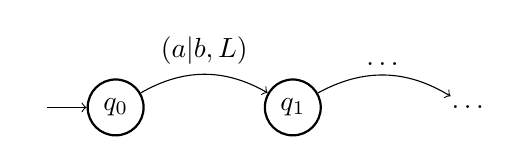
\begin{tikzpicture}[node distance=2.25cm,auto]
	\node(q0)[draw,circle,thick]{$q_0$};
	\node (s) [node distance=1cm,left of =q0]{};
	\node(q1)[draw,circle,thick,right of=q0]{$q_1$};
	\node(qx)[right of=q1]{\dots};

	\path[->]       (s) edge (q0)
	                (q0) edge[bend left] node{$(a|b,L)$} (q1)
			                (q1) edge[bend left] node{\dots} (qx);
					\end{tikzpicture}
					\end{center}

					Dabei steht die Kantenbeschriftung ``$(a|b,L)$'' für den Übergang $\delta(q_0,a) =
					(q_1,b,L)$.

					\vspace{2mm}
					Falls es für einen gegebenen Zustand und ein gegebenes
					Symbol keinen Zustandsübergang gibt, bricht die Maschine die Berechnung ab. 
}


\begin{frame}
\frametitle{Turingmaschine}
 \label{sec:busy_beaver}

Konstruieren Sie eine Turingmaschine, die aus drei Zuständen (plus einem
weiteren Haltezustand $q_f$) besteht und folgendes Verhalten hat:
\begin{quote}
  Angesetzt auf ein leeres Band schreibt sie möglichst viele ${\tt 1}$
  hintereinander und \textbf{hält} nach endlich vielen Schritten.
\end{quote}
Die Turingmaschine soll folgende Alphabete verwenden: $\Sigma = \{{\tt 1}\},
\Gamma = \Sigma \cup \{{\tt 0}\}$.  Insbesondere ist also ${\tt 0}$ das
Blanksymbol.

Welche Konfigurationen durchläuft die Maschine, wenn Sie auf dem leeren Band
gestartet wird?  Welche Konfigurationen durchläuft die Maschine bei Eingabe
des Wortes {\tt 101}?
\end{frame}
\begin{frame}
 Geben Sie eine wohldokumentierte Turingmaschine an, die zwei durch Blank
getrennte Binärworte aus $\{0,1\}^*$ addiert.
\end{frame}

%Entscheidbarkeit
\section*{}
\begin{frame}
 \frametitle{Definitionen zur TM (Vorlesung)}
 \begin{enumerate}
  \item Eine TM \emph{akzeptiert} eine Eingabe $w \in \Sigma^*$, wenn sie nach Lesen von $w$ in einem Zustand aus $F$ stoppt.
  \item Sie \emph{akzeptiert} eine Sprache $L \subseteq \Sigma^*$ genau dann, wenn sie ausschließlich Wörter $w$ aus $L$ als Eingabe akzeptiert.
  \item Eine Sprache $L \subseteq \Sigma^*$ heißt \emph{rekursiv} oder \emph{entscheidbar}, wenn es eine Turingmaschine gibt, die auf allen Eingaben stoppt und
	ein Wort $w \in \Sigma^*$ genau dann akzeptiert, wenn $w \in L$ gilt.
  \item Eine Sprache $L \subseteq \Sigma^*$ heißt \emph{rekursiv-aufzählbar} oder \emph{semi-entscheidbar}, wenn es eine Turingmaschine gibt, 
	die genau $w$ genau dann akzeptiert, wenn $w \in L$ gilt. Das Verhalten der Turingmaschine für Eingaben $w \not\in L$ ist damit nicht definiert.
	Sie stoppt entweder nicht in einem Endzustand oder aber stoppt garnicht.
 \end{enumerate}
\end{frame}

\begin{frame}
 \frametitle{Beispiel zur Akzeptanz}
 \begin{itemize}
  \item $\Sigma := \{a, b\}$  
  \item $F := \{q_4\}$
 \end{itemize}
\vspace{-2cm}
 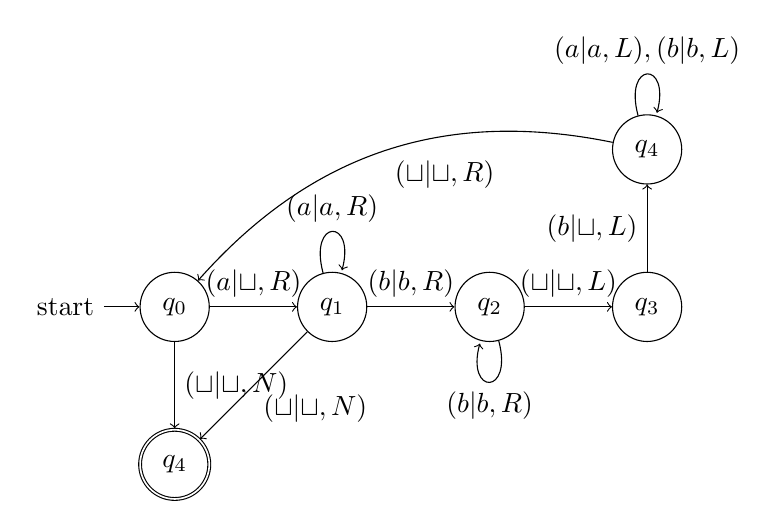
\begin{tikzpicture}[node distance=2cm,auto]
  \node(q0)[state,initial]{$q_0$};
  \node(q1)[state,right of=q0]{$q_1$};
  \node(q2)[state,right of=q1]{$q_2$};
  \node(q3)[state,right of=q2]{$q_3$};
  \node(q4)[state,above of=q3]{$q_4$};
  \node(q5)[state,accepting,below of=q0]{$q_4$};
  \path[->]       (q0) edge node{$(a|\sqcup,R)$} (q1)
	          (q0) edge node{$(\sqcup|\sqcup,N)$} (q5)
	          (q1) edge[loop above] node{$(a|a,R)$} ()
	          (q1) edge node{$(b|b,R)$} (q2)
	          (q1) edge node{$(\sqcup|\sqcup,N)$} (q5)
	          (q2) edge[loop below] node{$(b|b,R)$} ()
	          (q2) edge node{$(\sqcup|\sqcup,L)$} (q3)
	          (q3) edge node{$(b|\sqcup,L)$} (q4)
	          (q4) edge[loop above] node{$(a|a,L), (b|b,L)$} ()
	          (q4) edge[bend right] node{$(\sqcup|\sqcup,R)$} (q0);
 \end{tikzpicture}
 \end{frame}

\begin{frame}
 \frametitle{Sprache}
 \begin{itemize}
  \item $aab$ wird von der TM akzeptiert.
  \item $abb$ nicht.
  \item Die akzeptierte Sprache ist $L(TM) := \{a^kb^l| k >= l\}$
  \item Die Sprache ist offensichtlich semi-entscheidbar.
  \item Ist sie auch entscheidbar?
 \end{itemize}
\end{frame}


%TODO Beispiel für nicht entscheidbare Probleme
%TODO Beispiel für Entscheidbarkeit

\begin{frame}
\frametitle{Universelle Turingmaschine}
\begin{block}{Gödelnummer}
Jede Turingmaschine lässt sich eindeutig als Zahl kodieren. Eine solche Kodierung einer Turingmaschine nennen wir eine Gödelnummer dieser Turingmaschine. Wir vereinbaren weiterhin, dass alle gemäß unserer Kodierung ungültigen Gödelnummern einer TM zugeordnet werden, die alle Eingaben ablehnt.
\end{block}
\begin{block}{Universelle Turingmaschine}
Es existieren Turingmaschinen, die jede andere Turingmaschine bei Angabe der Entsprechenden Gödelnummer (also einer Kodierung), simulieren können. Diese TM erhält als Eingabe die Kodierung einer TM sowie eine Eingabe für die zu simulierende TM, und gibt die Ausgabe der simulierten TM aus.
\end{block}
\end{frame}

\begin{frame}
 \frametitle{Nicht entscheidbare Sprache}
 \begin{block}{Beispiel}
 \begin{itemize}
  \item Die Sprache aller ``Busy-Beaver''-Turingmaschinen mit 15 Zuständen ist nicht entscheidbar.
  \item Warum nicht?
 \end{itemize}
 \end{block}
\end{frame}

\begin{frame}
\frametitle{Aufgaben zur Entscheidbarkeit}
 Seien $L_1$ und $L_2$ zwei Sprachen über einem Alphabet $\Sigma$.
Beweisen Sie:
\begin{enumerate}
\item Ist $L_1$ entscheidbar, so ist auch $L_1^c$ entscheidbar.
\item Sind $L_1$ und $L_2$ entscheidbar, so ist auch $L_1\cup L_2$ entscheidbar.
\item Sind $L_1$ und $L_2$ entscheidbar, so ist auch $L_1\backslash L_2$ entscheidbar.
\item Ist $L_1$ entscheidbar, so ist auch die Sprache 
$$\min(L_1):=\{x\in L_1\mid \text{kein echtes Präfix von $x$ ist in }L_1 \}$$
entscheidbar.
\end{enumerate}
\end{frame}

\section*{}
\begin{frame}
 \frametitle{Aufgabe zur Semi-Entscheidbarkeit}
Sei $L$ eine semi-entscheidbare Sprache, die nicht entscheidbar ist. Ist die
Sprache $L'=\{0w:w \in L\} \cup \{1w: w \not\in L\}$ entscheidbar,
semi-entscheidbar oder keins von beiden?

Hinweis: Nimm an, $L'$ sei semi-entscheidbar, und folgere daraus, dass
dann $L$ entscheidbar ist. 
\end{frame}


\begin{frame}
 \frametitle{Halteproblem}
 Zeigen Sie, dass das Halteproblem semi-entscheidbar ist.
\end{frame}

% TM Erweiterungen
\begin{frame}
\frametitle{Erweiterungen von Turingmaschinen}
\begin{block}{Erweiterungen}
Es gibt mehrere, zu Turingmaschinen (bzgl. Berechenbarkeit) äquivalente Berechnungsmodelle, die der Turingmaschine sehr ähnlich sind. Man spricht hier von Erweiterungen von Turingmaschinen. Diese verwendet man gerne in z.B. Beweisen, da sie oft Übersichtlicher sind.
\end{block}
\end{frame}
% Mehrkopf
\begin{frame}
\frametitle{Mehrkopf-Turingmaschinen}
\vspace{-2cm}
\begin{figure}[H]
\begin{center}
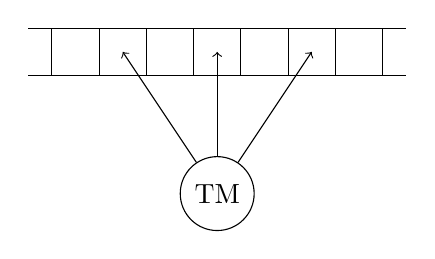
\begin{tikzpicture}[scale=0.3]
\draw (-8,1) -- (8,1);
\draw (-8,-1) -- (8,-1);
\draw (7,1) -- (7,-1);
\draw (5,1) -- (5,-1);
\draw (3,1) -- (3,-1);
\draw (1,1) -- (1,-1);
\draw (-1,1) -- (-1,-1);
\draw (-3,1) -- (-3,-1);
\draw (-5,1) -- (-5,-1);
\draw (-7,1) -- (-7,-1);
\node[draw,circle] (tm) at (0,-6) {TM};
\draw[->] (tm) -- (0,0);
\draw[->,bend left] (tm) -- (-4,0);
\draw[->,bend right] (tm) -- (4,0);
\end{tikzpicture}
\end{center}
\end{figure}
Eine Mehrkopf-Turingmaschine hat mehrere Lese-/Schreibeköpfe. Die Zustandsänderung hängt nun von dem gelesenen Zeichen aller Köpfe ab und kann auch alle Köpfe verschieben bzw. mit allen gleichzeitig schreiben.
\begin{block}{Änderungen in der Definition}
$$ \delta: Q \times \Gamma^n \rightarrow Q \times \Gamma^n \times \{L,N,R\}^n$$
\end{block}
\end{frame}

% Mehrband
\begin{frame}
\frametitle{Mehrband-Turingmaschinen}
\vspace{-2cm}
\begin{figure}[H]
\begin{center}
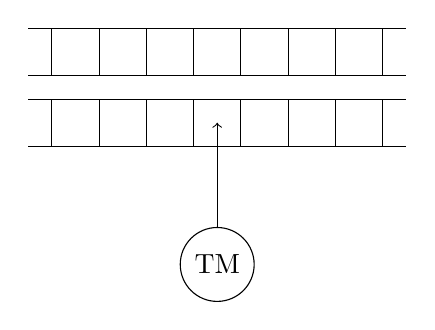
\begin{tikzpicture}[scale=0.3]
\draw (-8,4) -- (8,4);
\draw (-8,2) -- (8,2);
\draw (7,4) -- (7,2);
\draw (5,4) -- (5,2);
\draw (3,4) -- (3,2);
\draw (1,4) -- (1,2);
\draw (-1,4) -- (-1,2);
\draw (-3,4) -- (-3,2);
\draw (-5,4) -- (-5,2);
\draw (-7,4) -- (-7,2);

\draw (-8,1) -- (8,1);
\draw (-8,-1) -- (8,-1);
\draw (7,1) -- (7,-1);
\draw (5,1) -- (5,-1);
\draw (3,1) -- (3,-1);
\draw (1,1) -- (1,-1);
\draw (-1,1) -- (-1,-1);
\draw (-3,1) -- (-3,-1);
\draw (-5,1) -- (-5,-1);
\draw (-7,1) -- (-7,-1);

\draw (-8,1) -- (8,1);
\draw (-8,-1) -- (8,-1);
\draw (7,1) -- (7,-1);
\draw (5,1) -- (5,-1);
\draw (3,1) -- (3,-1);
\draw (1,1) -- (1,-1);
\draw (-1,1) -- (-1,-1);
\draw (-3,1) -- (-3,-1);
\draw (-5,1) -- (-5,-1);
\draw (-7,1) -- (-7,-1);
\node[draw,circle] (tm) at (0,-6) {TM};
\draw[->] (tm) -- (0,0);
\end{tikzpicture}
\end{center}
\end{figure}
Eine Mehrband-Turingmaschine hat mehrere Bänder. Die Zustandsänderung kann nun auch auf ein anderes Band wechseln. Dabei wird immer auf die zuletzt eingenommene Position auf dem anderen Band gewechselt 
\begin{block}{Änderungen in der Definition}
$$ \delta: Q \times \Gamma \times \{1, \ldots, n\} \rightarrow Q \times \Gamma \times \{L,N,R\} \times \{1, \ldots, n\}$$
\end{block}
\end{frame}
% Mehrdim
\begin{frame}
\frametitle{Mehrkopf Turingmaschinen}
\vspace{-2cm}
\begin{figure}[H]
\begin{center}
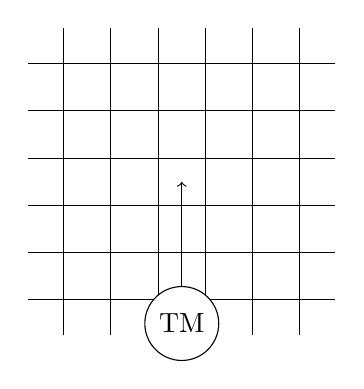
\begin{tikzpicture}[scale=0.3]
\draw[step=2cm,xshift=1cm,yshift=1cm] (-7.5,-7.5) grid (5.5,5.5);
\node[draw,circle,fill=white] (tm) at (0,-6) {TM};
\draw[->] (tm) -- (0,0);
\end{tikzpicture}
\end{center}
\end{figure}
Eine Mehrdimensionale Turingmaschine hat ein Mehrdimensionales Band, der Kopf kann sich dann in allen verfügbaren Dimensionen bewegen.
\begin{block}{Änderungen in der Definition (für Dimension 2)}
$$ \delta: Q \times \Gamma \rightarrow Q \times \Gamma \times \{L,N,R,U,D\}$$
\end{block}
\end{frame}

% Beispiel (if time)
% Aufgabe
\begin{frame}
\frametitle{Aufgabe}
\vspace{-1cm}
Eine $k$-Band-Turingmaschine ist eine Turingmaschine mit $k$
Arbeitsbändern und der Übergangsfunktion

\[ \delta: Q \times \Gamma \times \{1, \ldots, k\} \to
Q \times \Gamma \times \{L, R, N\} \times \{1, \ldots, k\}, \]

wobei $\delta(q, a, i) = (p, b, X, j)$ bedeute:

\begin{quote}
  Wenn sich die Maschine im Zustand $q$ befindet und
  auf Band $i$ das Symbol $a$ liest, so springt die Maschine in Zustand $p$,
  überschreibt $a$ mit $b$, der Lese-Schreib-Kopf bewegt sich auf Band $i$
  gemäß $X$ und springt auf Band $j$ an die Stelle, an der er sich
  auf diesem Band zuletzt befunden hat.
\end{quote}

Die Eingabe befinde sich auf Band 1, und im Zustand $s$ befinde sich der
Kopf an der ersten Stelle der Eingabe. Die Stelle, auf die der Kopf bei einem
Wechsel auf ein bis dahin unbenutztes Band springt, sei
festgelegt.
Eine solche 2-Band-Turingmaschine habe nun Zeitaufwand $T(n)$.
Zeigen Sie informell, dass diese von einer einfachen
Turingmaschine mit Zeitaufwand $O(T^2(n))$ simuliert werden kann.\\
\end{frame}

% Satz von Rice
\begin{frame}
\frametitle{Satz von Rice}
Der Satz von Rice sagt aus, dass es unmöglich ist eine nichttriviale Eigenschaft von Turingmaschinen algorithmisch zu entscheiden.
\begin{block}{Formale Version}
Es sei R die Klasse aller Turing-berechenbaren Funktionen und $S$ eine beliebige nichttriviale (das bedeutet $S \neq \emptyset$ und $S \neq R$) Teilmenge davon. Dann ist die Sprache
$$ C_S = \{ i |\text{ die von $M_i$ berechnete Funktion liegt in $S$} \} $$
Unentscheidbar. 
\end{block}
\end{frame}
% Beispiel
\begin{frame}
\frametitle{Beispiel}
Die Klasse aller Programme die etwas auf einem Rechner tun, das der Benutzer nicht möchte (das ist eine Teilmenge der Turingberechenbaren Funktionen) ist unentscheidbar. Daraus folgt, dass es keinen perfekten Virenscanner geben kann!
\end{frame}

% Aufgabe
\begin{frame}
\frametitle{Aufgabe}
Kann man die Entscheidbarkeit der folgenden Mengen mithilfe des Satzes von Rice bestimmen?
\begin{itemize}
\item Alle Turingmaschinen die nur $0$ aufs Band Schreiben.
\item Alle Turingmaschinen die im ersten Schritt genau eine $0$ aufs Band Schreiben und im zweiten Schritt anhalten. 
\item Alle Turingmaschinen die überhaupt etwas auf das Band schreiben.
\end{itemize}
\end{frame}
\begin{frame}
\frametitle{Postsches Korrespondenzproblem}
Gegeben sei einer Folge von Paaren $((x_1, y_1), (x_2, y_2), \ldots, (x_n,y_n))$ von nichtleeren Worten über einem endlichen Alphabet. Dies nennt man eine \textbf{Instanz} des PKP.
Eine nicht-leere Folge $I = i_1, i_2, \ldots, i_m$ von indices $\{1, \ldots, n\}$ heißt Lösung zu $P$, wenn $x_{i_1}x_{i_2}\ldots{}x_{i_m} = y_{i_1}y_{i_2}\ldots{}y_{i_m}$.
\begin{block}{Beispiel}
\begin{displaymath}
\{ {a \choose aba}, {ab \choose bb}, {baa \choose aa} \}
\end{displaymath}

Lösung: $1,3,2,3$
\begin{displaymath}
{a \choose aba}, {baa \choose aa}, {ab \choose bb}, {baa \choose aa}
\end{displaymath}

\end{block}
\end{frame}

\begin{frame}
\frametitle{Aufgabe}
\begin{enumerate}
\item Finde eine Lösung für folgende Instanz des Post'schen Korrespondenzproblems: 
\[ ((aa, a), (b, aa), (a, aab)) \]
  \item Zeigen Sie, dass folgende Instanz des Post'schen Korrespondenzproblems
        keine Lösung hat:

        \[ ((ab, b), (bba, abb), (ab, ba), (a, abb)) \]

  \item Zeigen Sie, dass das Post'sche Korrespondenzproblem für Wörter
über einem Alphabet mit nur einem Symbol entscheidbar ist.
\end{enumerate}
\end{frame}

\begin{frame}
\frametitle{Aufgabe}
Finde eine Lösung für folgendes PCP
$$ ((001,0),(01,011),(01,101),(10,001)) $$
\pause
Eine kürzeste Lösung hat mindestens die Länge 66, z.B:
\begin{center}
$ I_1 = $(2,4,3,4,4,2,1,2,4,3,4,3,4,4,3,4,4,2,1,4,\\
4,2,1,3,4,1,1,3,4,4,4,2,1,2,1,1,1,3,4,3,4,1,2,\\
1,4,4,2,1,4,1,1,3,4,1,1,3,1,1,3,1,2,1,4,1,1,3)
\end{center}
\end{frame}

%TODO: Definition + Beispiel zu Optimierungsproblemen
\begin{frame}
 \frametitle{Optimierungsproblem}
 Gegeben sei ein Graph $G=(V,E)$ mit $V:=\{1,\ldots,n\}$ und $E\subseteq \{\{u,v\} \mid u,v \in V, u\neq v\}$. Weiter seien $c:E \rightarrow \mathbb{R}^+$ eine Längenfunktion auf den Kanten des Graphen sowie $s\in V$ ein ausgewiesener Start- und $t\in V$ ein ausgewiesener Zielknoten. 
Ein Pfad von $s$ nach $t$ ist eine Folge von Kanten $p = \{i_1,i_2\},\{i_2,i_3\},\ldots,\{i_{k-2},i_{k-1}\},\{i_{k-1},i_k\}$ mit $\{i_j, i_{j+1}\} \in E$ und $i_1=s$ sowie $i_k=t$. 
Die Länge des Pfades sei definiert als die Summe der Längen aller Kanten auf dem Pfad. 
Betrachten Sie die Menge der Pfade, die von $s$ nach $t$ führen, und formulieren Sie ein naheliegendes Optimierungsproblem. 
Formulieren Sie ein zu Ihrem Optimierungsproblem gehörendes Entscheidungsproblem.
\end{frame}

%TODO Definition zu Kodierungsschemata

\begin{frame}
 \frametitle{Kodierungsschemata (VL)}
 \begin{block}{Definition Kodierungsschemata}
 Ein \emph{Kodierungsschema} s ordnet jedem Problembeispiel eines Problems eine Zeichenkette oder Kodierung über einem Alphabet $\Sigma$ zu. 
 Die Inputlänge eines Problembeispiels ist die Anzahl der Symbole seiner Kodierung.
 Dabei gibt es natürliche verschiedene Kodierungsschemata für ein bestimmtes Problem.
 \end{block}
\end{frame}

\begin{frame}
 \frametitle{Kodierungsschemata}
 Das Entscheidungsproblem \textit{PRIMES} besteht darin, zu entscheiden, ob es sich bei einer gegebenen natürlichen Zahl $p>1$ um eine Primzahl handelt. 
Eine Probleminstanz von \textit{PRIMES} wird also durch eine natürliche Zahl kodiert. 
Für $b\in \mathbb{N}$ bezeichne $s_b$ das Kodierungsschema, welches Zahlen zur Basis $b$ darstellt.

Zeigen Sie, dass die Kodierungsschemata $s_a$ und $s_b$ für $a,b>1$ bezüglich \textit{PRIMES} äquivalent sind.
\end{frame}

% TM klasse P
\begin{frame}
\frametitle{Die Klasse $\mathcal{P}$}
Die Klasse $\mathcal{P}$ ist definiert als die Menge aller Sprachen, die von einer (deterministischen) Turingmaschine, deren Zeitkomplexität höchstens polynomial ist, entschieden werden können.
\end{frame}

\begin{frame}
\frametitle{Sind folgende Sprachen in $\mathcal{P}$?}
\begin{itemize}
\item Die Wörter der deutschen Sprache
\item Die ungraden Zahlen
\item Eine reguläre Sprache $L$
\item Die PCPs die eine Lösung haben
\item Die unär kodierten Primzahlen
\item Die binär kodierten Primzahlen
\end{itemize}
\end{frame}

%\begin{frame}
%\frametitle{Bekannte Sprachen in \mathcal{P} sind:}
%\begin{itemize}
%\item 2-Färbbare Graphen
%\item Existenz eines Eulerzykluses
%\end{itemize}
%\end{frame}

\begin{frame}
 \frametitle{Laufzeitbetrachtung}
 Betrachten Sie $L_1 := L[\text{\textit{PRIMES}},s_1]$. 
Ein naiver Algorithmus für \textit{PRIMES} könnte alle Zahlen $2,3,\ldots,p-1$ darauf hin überprüfen, ob sie die gegebene Zahl $p$ teilen. 
Beschreiben Sie kurz in Worten die Arbeitsweise einer \textbf{deterministischen} Turing-Maschine, die diesen Algorithmus implementiert und damit $L_1$ entscheidet. 
Geben Sie die Laufzeit Ihrer Turing-Maschine asymptotisch an. Ist $L_1$ in $\mathcal{P}$? Begründen Sie gegebenenfalls, warum $L_1$ in $\mathcal{P}$ ist.
\end{frame}

% NDTMs mit Orakelmodul
% Kurz angesprochen andere Definitionen:
%% TM mit Nichtdeterministischen übergängen
% Konzept TM mit "lösungsrater und Verifier"
% NP als Klasse
% co-NP?
% NP vollständigkeit
% Polyreduktionen
% Polytransformationen mit NPCness

\begin{frame}
\frametitle{$\mathcal{NP}$}
 Betrachten Sie die Sprache $L_{10}^c := L[\text{\textit{PRIMES}},s_{10}]^c$ der \textit{zusammengesetzten} Zahlen in Dezimaldarstellung. 
Beschreiben Sie grob in Worten die Arbeitsweise einer \textbf{nichtdeterministischen} Turing-Maschine, die $L_{10}^c$ entscheidet. 
Ein Unterprogramm für die Division von Dezimalzahlen mit polynomieller Laufzeit sei gegeben und kann von Ihrer Turing-Maschine aufgerufen werden. 
Ist $L_{10}^c$ in $\mathcal{NP}$? Begründen Sie gegebenenfalls, warum $L_{10}^c$ in $\mathcal{NP}$ ist.

\medskip
\textit{Hinweis:} Überlegen Sie sich, was Ihre Turing-Maschine in der Orakel-Phase sinnvollerweise auf das Band schreiben könnte.
\end{frame}


\frame{
  \frametitle{Lizenzen}
  \center
  
\includegraphics[width=2em]{images/by}
  
\includegraphics[width=2em]{images/cc}
  
\includegraphics[width=2em]{images/sa}
  \\
  {\tiny

Dieses Werk ist unter einem Creative Commons Namensnennung-Weitergabe unter gleichen Bedingungen 3.0 Deutschland Lizenzvertrag lizenziert. Um die Lizenz anzusehen, gehen Sie bitte zu \href{http://creativecommons.org/licenses/by-sa/3.0/de/}{http://creativecommons.org/licenses/by-sa/3.0/de/} oder schicken Sie einen Brief an Creative Commons, 171 Second Street, Suite 300, San Francisco, California 94105, USA.\\
  \vspace{1cm}
  Davon ausgenommen sind das Titelbild, welches aus der März-April 2002 Ausgabe von American Scientist erschienen ist und mit Erlaubnis verwendet wird, sowie das KIT Beamer Theme. Hierfür gelten die Bestimmungen der jeweiligen Urheber.
  \vspace{1cm}
  \\ 
  Dank an 
  Moritz v. Looz und 
  Simon Stroh,
  deren LaTeX-Quellen zum Erstellen dieser Folien verwendet wurden.
  }%Add whoever contributes
  %Habe hier die Reihenfolge etwas umgestellt, weil die Formatierung bei mir komisch aussah. 
  %Wenn es bei dir anders ist, kannst du es auch wieder zurückändern, dann haben wir unterschiedliche Kompilieroptionen
  %Sollen wir uns wirklich selbst danken?
}

\end{document}
